% This thesis is built on the belief that ...
% This chapter evaluates the  ...

In this chapter, we aim to validate our analysis of the trade-offs involved in query processing state placement decisions,
and to evaluate the effectiveness of our design and prototype implementation in providing an effective mechanism to applications
for navigating these trade-offs.

The aim of this evaluation is to answer the following questions:

\begin{itemize}

  \item What improvements in query processing performance can be achieved by placing materialized state close to clients?
  (Section~\ref{sec:eval_query_processing_perf})

  \item When materialized state is placed close to the data storage tier,
  how does Proteus compare to an approach in which materialized state is maintained by the data storage tier itself?
  (Section~\ref{sec:eval_query_processing_perf})

  \item What are the penalties in freshness resulting from placing materialized state away from the data storage tier?
  (Section~\ref{sec:eval_freshness_throughput})

  \item How does freshness scale as the load of the system increases? (Section~\ref{sec:eval_freshness_throughput})

  \item What is the overhead of the micro-service architecture in freshness? (Section~\ref{sec:eval_freshness_throughput})

  \item How does round-trip time between sites affect freshness? (Section~\ref{sec:eval_freshness_rtt})

  \item What additional data transfer costs result from materialized state placed close to clients receiving updates?
  (Section~\ref{sec:eval_data_transfer})

\end{itemize}


\section{Experimental scenario}

The evaluation in this chapter is based on the case study presented in Section~\ref{sec:lobsters},
which describes the Lobsters \cite{lobste:rs} web application.
We have chosen this application because it is characterized by a read-heavy workload that requires the materialization
of derived state.
Moreover, the derived state is updated by a stream of small updates.
These characteristics make Lobsters suitable for evaluating the efficacy of our design and prototype implementation in
navigating the trade-offs of query processing state placement.
In addition, the Lobsters application is open-source \cite{lobsters:source},
allowing us to examine the application's interaction with the database,
and statistics about the applications data distributions and access patterns are available \cite{lobste:stats}.
Finally, Lobsters resembles a class of popular large-scale web applications, such as Reddit and Hacker News.

\bigskip
\noindent
In Lobsters, users post, comment, and vote on ``stories''.
Each story is associated with a ``hotness'' value that indicates how popular it is.
Stories are ranked based on their hotness;
the highest ranked stories appear on the front page.
The hotness value of a story depends on parameters such as the number of votes a story has gotten,
the number of comments, and the hotness of those comments.
As a result, various operations, such as voting or commenting on a story, modify its hotness value.
It is prohibitively expensive \cite{gjengset:noria} to compute the hotness value of stories during queries.
In particular, serving the Lobsters' front page requires computing the hotness of every story in order to rank them.
That is why the Lobsters application instead adds an additional column to the $stories$ table (the Lobsters application
uses MySQL for storing its state) which stores the computed hotness value for each story.
The application updates the value of the hotness column when operations such as upvoting or downvoting a story, or
adding a comment to a story are performed.

For this evaluation, we consider a simplified version of the Lobsters application.
In particular, we consider the following database schema:

\begin{lstlisting}[
          language=SQL,
          showspaces=false,
          basicstyle=\ttfamily,
          commentstyle=\color{gray},
          rulecolor=\color{black},
          stringstyle=\color{mymauve},
          frame=L,
          xleftmargin=\parindent,
          commentstyle = \color{gray}
        ]
TABLE users (id bigint, username varchar(50))
TABLE stories (id bigint, user_id bigint, title varchar(150), description mediumtext, short_id varchar(6));
TABLE votes (id bigint, user_id bigint, story_id bigint, vote tinyint);
\end{lstlisting}

In addition, we consider a workload consisting of two operations: voting up or down a given story and requesting the Lobsters
front page.
The front page is a listing of the 25 most highly ranked stories, including their title, author, and vote count.
In the statistics provided by the Lobsters administrators, the front page operation constitutes 30.1\% of client requests,
and voting on stories constitutes 0.5\% of client requests.
Our simplified workload consists of 95\% front page operations, and 5\% voting operations, unless otherwise specified.

This restricted application model gives as better control over the properties of the workload for the purposes of
this evaluation,
while also capturing the aspects of the Lobsters application that make it suitable for use in this evaluation.


\begin{table}[H]
\centering
\begin{tabular}{|c||c|c|c|c|c|c|}
\hline
Number of votes & [0-10) & [10-20) & [20-30) & [30-40) & [40-50) & [50-60) \\
\hline
\% of stories & 41.1 & 40.3 & 11.3 & 4.2 & 1.6 & 1.3 \\
\hline
\end{tabular}
\caption{Distribution of votes to stories in the Lobsters statistics available at \cite{lobste:stats}}
\label{tab:votes_per_story}
\end{table}

The statistics provided by the maintainers of Lobsters \cite{lobste:stats} include the distribution of votes to stories (Table~\ref{tab:votes_per_story}).
As expected, most stories (81.4\%) receive between 0 and 20 votes.
For our experiments, we use a more skewed (and less realistic) distribution:
We configure 60\% of votes to target the 25 stories in the frontpage, and 40\% to follow the distribution shown in Table~\ref{tab:votes_per_story}.
We choose this distribution because our initial benchmarks showed that with votes following the distribution given by the statistics,
very few votes are performed on the stories on the front page to have meaningful impact on freshness.

\begin{figure}[H]
  \centering
    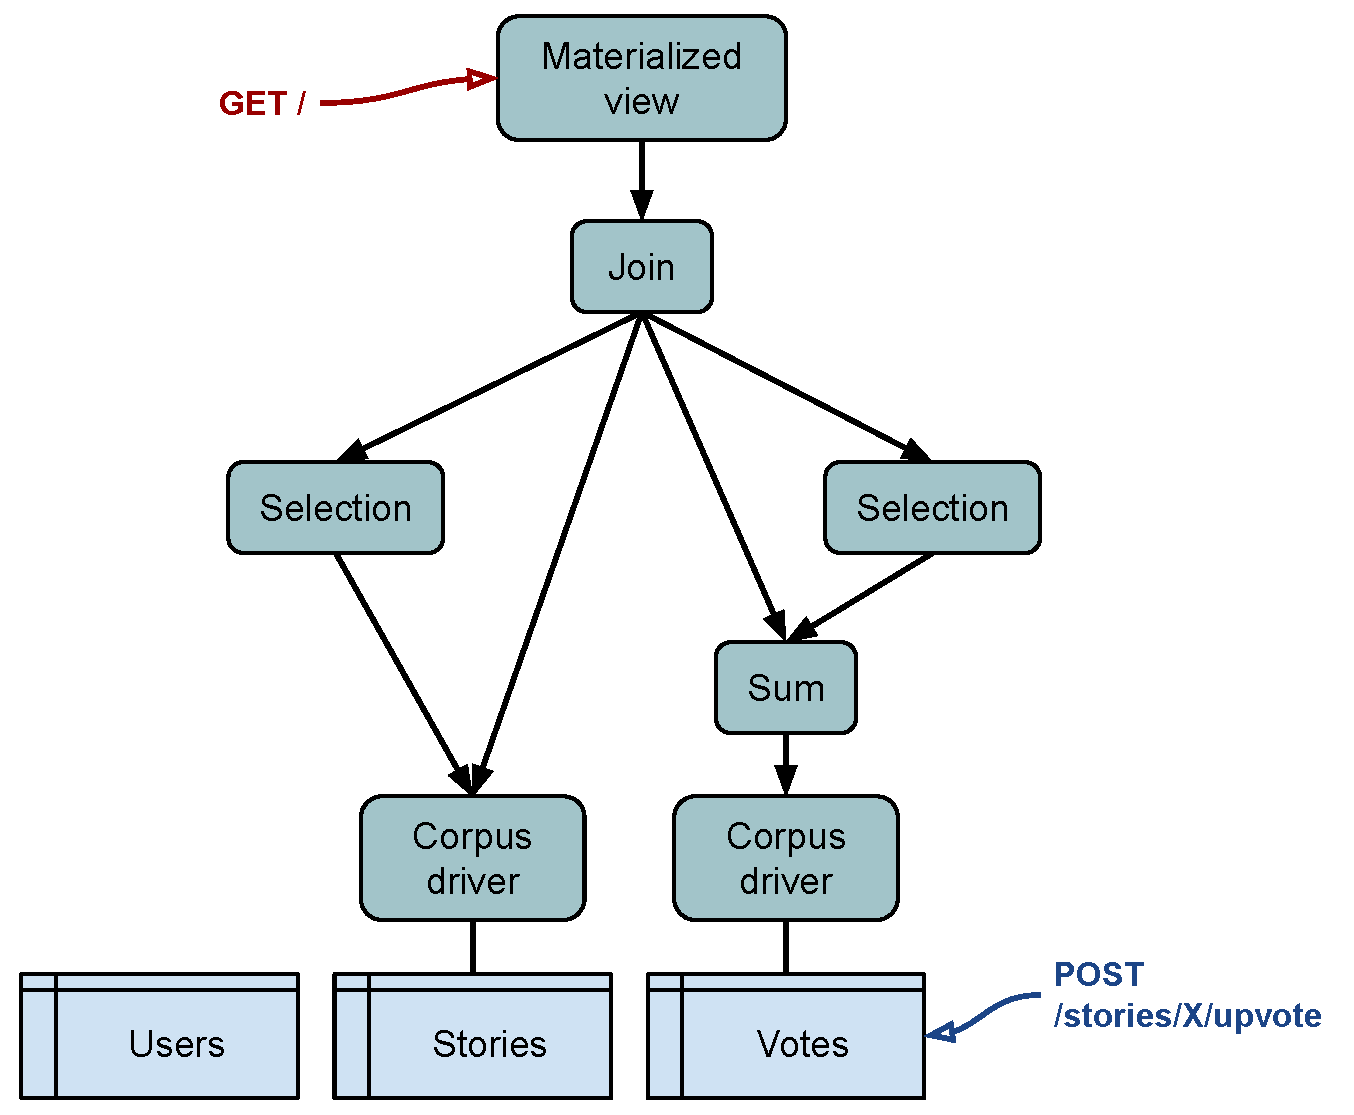
\includegraphics[scale=0.5]{./figures/evaluation/lobsters_architecture_eval.pdf}
  \caption{QPU architecture used for this evaluation. The Materialized view QPU integrates stories with vote counts.
  The ``GET /'' request indicates the front page operation, and the ``POST /stories/X/upvote'' request indicates the operation of voting up for story X.}
  \label{fig:eval_lobsters_qpu_arch}
\end{figure}

\bigskip
\noindent
The evaluation uses the QPU architecture depicted in Figure~\ref{fig:eval_lobsters_qpu_arch}.
This architecture maintains a materialized view that integrates stories from the $stories$ table,
with their vote count.
The view definition the following query:

\begin{lstlisting}[
          language=SQL,
          showspaces=false,
          basicstyle=\ttfamily,
          commentstyle=\color{gray},
          rulecolor=\color{black},
          stringstyle=\color{mymauve},
          frame=L,
          xleftmargin=\parindent,
          commentstyle = \color{gray}
        ]
SELECT id, author_id, title, url, vote_count
FROM stories
JOIN (
  SELECT story_id, SUM(vote) as vote_count
  FROM votes
  GROUP BY story_id
) view
ON stories.id = view.story_id
\end{lstlisting}

This simplifies both the vote and front page operations compared to the baseline Lobsters implementation:
the vote operation does not need to explicitly update the hotness (here the vote count) of the given story as this
is performed by the QPU graph,
and the front page operation can be served from the materialized view.

In the actual QPU graph deployed for the experiments, Selection QPUs are merged with their downstream connections.
More generally, in our implement the Selection QPU is merged with every other QPU class,
as it is commonly used and can be implemented by a simple filter function.
In addition, the Materialized View is merged with the Join QPU.

The Materialized view QPU implementation used in these experiments stores its state in a MySQL instance.
This is a separate MySQL instance from the one that is used the Lobsters database.
It is deployed alongside and only accessible by the Materialized view QPU.
The choice of using the same database both as the baseline and for storing the materialized view is aimed at eliminating
the effect of the database performance from the evaluation results,
providing a comparison that isolates the effects of placement.

In addition, we use an index on the materialized view to support efficient retrieval of the stories with the highest vote count.

\bigskip
\noindent
We consider a system architecture consisting of two geographically distant sites:
The Lobsters application is deployed on one site (we henceforth refer to this site as application site),
and clients are located on another site (client site).
Round-trip time between these two sites is 80ms.
This corresponds to a scenario in which the Lobsters web application is deployed in a data centers in North America,
and clients are located in Europe \cite{pbailis:hats}, or vice versa.

In our experiments, we make use of the QPU graphs ability to be placed flexibly across the system.
We use two placement schemes:
One in which the root of the graph (Materialized view QPU) is placed on the application and one in which it is placed on
the client site.
We evaluate the effects and trade-offs of materialized view placement by comparing these two placement schemes.


\section{Experimental Setup}

This evaluation does not use the real Lobsters Ruby-on-Rails application.
Instead, we have implemented a adapter that translates user requests to queries that the real
Lobsters application would issue to the database,
and issues those queries either to MySQL, or MySQL and Proteus depending on the experiment configuration.
This allows us to isolate the interaction between the application and the database, which is the focus of this work,
and remove other tasks that the Lobsters application performs, which quickly become a bottleneck.

We have implemented this adapter as a server-side adapter:
it is deployed along with the database on the application site, and plays the role of a simplified web server:
It exposes a gRPC endpoint, similar to the QPU gRPC server, and clients issue operations to it as RPC requests.

\bigskip
\noindent
\textbf{Workload generation.}
For this evaluation, we have implemented a workload generator \cite{lobsters:bench} that is responsible for issuing
requests to the Lobsters adapter.
In addition, the workload generator measures the achieved throughput and operation response time.
We define response time as the delay that a client application experiences between issuing a request and receiving the
corresponding response.
To capture the variance of response time, we use a histogram data structure provided by the Go implementation of gRPC \cite{grpcgo:histogram}.
that accumulates values in a histogram with exponentially increasing bucket sizes, and enables us to compute response time percentiles.

The workload generator uses an open-loop model \cite{schroeder:cautionarytale}:
it creates requests based on a target load (requests submitted per second) value;
each request is executed by a separate thread (creating and destroying threads are low-cost operations because threads are
implemented as Goroutines).

The overall number of requests (and thus threads) that can be ongoing at a given point in time is bounded by a
configuration parameter.
When the bound is reached, additional requests need to wait for ongoing requests to be completed.
Our experiments showed this concurrency bound mechanism is essential for preventing a positive feedback loop effect
that takes place above a certain load threshold:
When the system starts not being able to handle the load, response time increases as a result.
However, the workload generator keeps generating requests, and, because of the increased response time,
more requests are ongoing concurrently, which puts more load in the gRPC server, increasing the load more.
As a result even a small initial increase in response time triggers this feedback loop,
which eventually increases response time more and more during the duration of the benchmark.

The concurrency bound mechanism is effective in avoiding this effect.
However, it also means that when running a benchmark for a given target load we need to specify a bound in the number of
concurrent threads that is sufficient for reaching the target load.
If the bound is too low, then the workload generator cannot generate enough load, but and but response time does not
increase because the delay caused by waiting for available threads is outside of the response time measurement.

\bigskip
\noindent
\textbf{Freshness.} The materialized state maintained by the Materialized view QPU eventually consistent
relative to the state of the Lobsters database.
As a result, queries served from the materialized view might reflect state that is stale relative to the database state.
The freshness of the materialized state is impacted by its placement:
Placing the Materialized view QPU at the client side entails that there is a 40ms communication latency for updates
sent to the materialized view.

One of the aims of this evaluation is to quantify how stale query results are.
To achieve that, we measure the freshness of the results returned by the front page operation.
We use two freshness metrics:
\begin{itemize}
  \item \textbf{Update latency:} The delay between a vote being committed in the database, and the materialized view being
  updated with the new vote count.
  \item \textbf{Returned version:} How stale the returned version of a story is, measured as the number of versions
  to the version that would have been read if querying the Lobsters database instead of the materialized view.
\end{itemize}

We have implemented the following mechanism to collect these two metrics.
For each vote operation, MySQL logs the timestamp at which the corresponding transaction is committed;
this timestamp is then propagated through the QPU graph as an attribute, and stored by the materialized view in an
``update log'' table.
Moreover, the Materialized view QPU logs the commit timestamp of each view update in update log,
and the timestamp at the start of each query (building a ``query log'')

At the end of a benchmark run, the Materialized view QPU performs a post mortem analysis:
The update latency for each vote is computed by subtracting the timestamp at which the materialized view was updates from
the timestamp at which the vote was committed in the database.
The returned version for each front page story is computed by replaying the update and query logs,
and, for each query, computing how stale (measured in number of versions) a story record was in the materialized view
compared to the same story record in the database, when the query was executed.

A limitation of this mechanism is that it requires comparing timestamps taken on different servers.
To address that, in the benchmarks in which we take freshness measurements,
we deploy all system components (Lobsters MySQL database, QPU graph, workload generator) on a single server.
Because containers on a host share a single OS kernel, all timestamps used for computing freshness metrics are based
on the host operating system's clock, and thus can be meaningfully compared.
As mentioned below, we use the Linux tc utility \cite{tc} to simulate the 80ms round-trip time between sites,
despite all containers being deployed on a single server.

\bigskip
\noindent
\textbf{Hardware.}
Experiments were run on a cluster located in Paris, provided by the Laboratoire d'Informatique de Paris 6 (LIP6).
Each server consists of 2 Intel Xeon E5645 CPUs, each with 6 cores, 64 GB RAM, an 128 GB SSD disk, and a 4 TB HDD disk.

\bigskip
\noindent
\textbf{Software.}
\todo{add versions}

\bigskip
\noindent
\textbf{Configuration.}
The average ping latency between servers in the cluster is less than 1ms.
We simulate the two geographically distant sites by using the Linux tc utility \cite{tc} to add delay to outgoing packets.

For response time measurements, the Lobsters MySQL instance and the QPU graph except the Materialized view QPU are deployed
on a single server on the application site, and the workload generator is on a server in the client site.
The Materialized view QPU is deployed on a separate dedicated server, either on the application or the client site,
according on the placement scheme being tested.
As described above, for the freshness measurements, all components are deployed on a single server.

Experiments run for 5 minutes unless otherwise specified, and we start taking measurements after an initial
``warmup period'' of 30 seconds.
Repeated runs have shown that results are stable and consistent across multiple runs.


\section{Query processing performance}
\label{sec:eval_query_processing_perf}
We compare three deployments that differ on how they store and calculate the per-story vote count,
and how they distribute computations and state across the nodes of the system.
\textbf{MySQL} is equivalent to the real Lobsters application:
it pre-computes and stores vote counts in a column of the Lobsters $stories$ table.
This serves as the baseline approach.
\textbf{Proteus-application} consists of the QPU graph shown in Figure~\ref{fig:eval_lobsters_qpu_arch},
deployed on the application site.
In \textbf{Proteus-client}, the Materialized view QPU is deployed on the client site while the rest of the graph
is deployed on the application site.
This is intended to evaluate the effect of placing the materialized view close the client.
We also compare with a deployment (\textbf{Materialized view internal}) in which the workload generator
directly issues request to the Materialized view QPU's state, bypassing the QPU's gRPC server
(the workload generator and materialized view are co-located on the same server).
This aims at providing an indication of the best performance the Materialized view QPU can achieve,
without taking into account its gRPC server (which we have identified as a performance bottleneck).

\begin{figure}[H]
\centering
  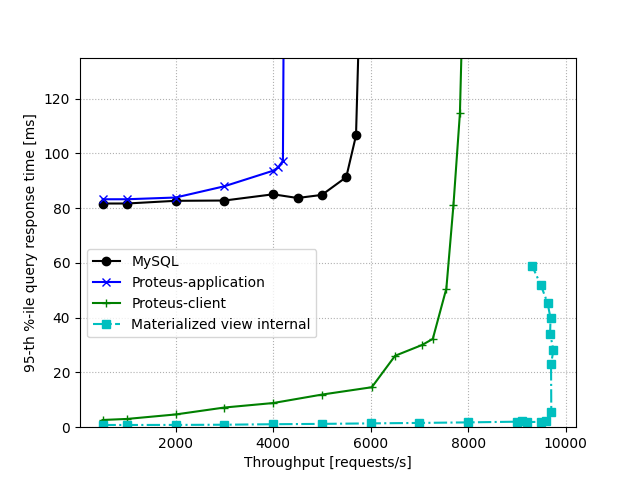
\includegraphics[width=0.7\textwidth]{./figures/evaluation/responseTime.png}
  \caption{Throughput vs 95th percentile query response time on a MySQL that resembles is similar to the real Lobsters application (MySQL), the Proteus deployment shown in Figure~\ref{fig:eval_lobsters_qpu_arch}
  with the Materialized view QPU placed on the application site (Proteus application), the same Proteus deployment with the Materialized view QPU placed on the client site (Proteus-client),
  and a setup in which the workload generator directly issues requests to the materialized view, bypassing the QPU's gRPC server (Materialized view internal).}
  \label{fig:responseTime}
\end{figure}

Figure~\ref{fig:responseTime} shows throughput -- query response time plots of these deployments.
The ideal throughput -- response time curve would be a horizontal line with low response time.
The lower bound response time for MySQL and Proteus-application is 80ms as this is the round-trip time between sites.
In reality, all systems' plots have a ``hockey stick'' shape:
latency remains relatively low until a point in which the system fails to keep up with the offered low.
After that point, the system cannot achieve additional throughput, and response time increases.

The plot of the Materialized view internal deployment indicates that that the Materialized view QPU can scale to 9800
requests/seconds when removing overheads other than the interaction with the database in which the materialized view is stored.
The Proteus-application and Proteus-client deployments have additional overheads and as a result scale to lower
throughput values.

Proteus-application scales to 4200 requests/second, which is a 24\% overhead compared to the baseline deployment (MySQL),
which scales to 5500 requests/second.
Both those deployments eventually read and write state to a MySQL instance, with a similar (but not identical) database scheme.
Their difference lies in the mechanism the use for translating requests to database accesses.
The adapter used in the MySQL deployment uses a simple logic that translates vote and front page request to database transactions.
Conversely, the  Materialized view QPU used in the Proteus-application deployment contains more complex logic,
which includes additional mechanisms,
such as parsing received queries in SQL form, and receiving records from its input stream and updating the materialized view.
We attribute the observed 24\% overhead to the more complex logic.

In the Proteus-client deployment, query response time is significantly lower.
This is achieved because moving the Materialized view QPU in the clients site removes the need for a costly round-trip to
the application site, and thus remove the 80ms lower bound.
In addition, Proteus-client achieves a 23\% increase in achieved throughput before response time exceeds 20ms.
We attribute this improvement to the lower concurrency required to generate the same load in Proteus-client
compared to Proteus-application and MySQL.
In more detail, offering a certain load (volume of requests/second) requires creating a number of concurrent client threads,
each performing a request.
When the round-trip time between sites is 80ms, each of these threads executes significantly longer compared to
when the round-trip is just a few milliseconds.
As a result, offering a given amount of load in the Proteus-application setup results in a significantly greater number
of threads, and thus open connections to the QPU's gRPC server, than in the Proteus-client setup.
If the number of connections that can be opened is not bounded by a connection pool, this overloads the QPU's gRPC server,
significantly increasing response times.
When a connection pool is used, each requests needs to wait for an available connection,
again increasing the end-to-end response time experienced by the client.

\medskip
\noindent
\textbf{Conclusion.} We have observed that placing materialized views closer to the client benefits read-heavy applications
by removing costly round-trip communication across sites, and achieves scalability improvements.


\section{Freshness}

\subsection{Freshness and Throughput}
\label{sec:eval_freshness_throughput}

\begin{figure}[H]
\centering
  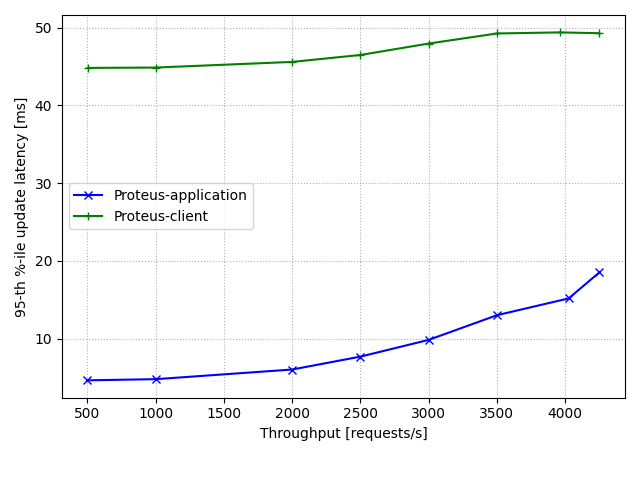
\includegraphics[width=0.7\textwidth]{./figures/evaluation/fr_latency_throughput.png}
  \caption{Throughput vs 95th percentile update latency.}
  \label{fig:fr_latency_throughput}
\end{figure}

Figure~\ref{fig:fr_latency_throughput} shows 95th percentile update latency as throughput increases,
for the Proteus-application and Proteus-client deployments.
AS described above, we define update latency as the delay between a vote being committed in the
Lobsters database, and the updated vote count being reflected in the materialized view.
The ideal throughput -- update latency curve would be a horizontal line with latency close to the lower bound defined by
the communication latency.
The lower bound for Proteus-application is 40ms while for Proteus-client it is less that 1ms.
In reality, latency remains low as long as the system can keep up with the offered vote request load,
and then increases.

Results show the Proteus-client setup scales well; Update latency remains within 5-10ms from the lower bound.
The Proteus-application setup exhibits a higher update latency:
For 4250 requests/second, the update latency in Proteus-application is 88\% higher than in Proteus-client,
relative to the lower bound.
This can be attributed to the same reasons as the scalability difference between the two deployments.

\begin{figure}[H]
\centering
  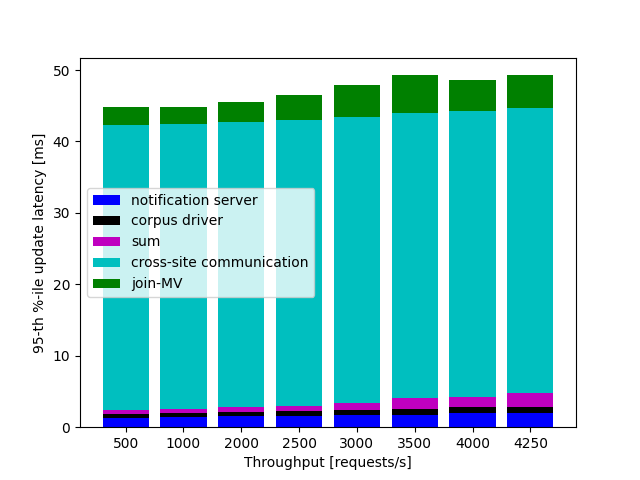
\includegraphics[width=0.7\textwidth]{./figures/evaluation/fr_latency_throughput_breakdown.png}
  \caption{Breakdown of 95th percentile update latency in the Proteus-client deployment
  (as shown in Figure~\ref{fig:fr_latency_throughput}) as throughput increases.}
  \label{fig:fr_latency_throughput_breakdown}
\end{figure}

Each vote committed in the database triggers a record that flows through the QPU graph, and eventually updates the corresponding
vote count in the Materialized view QPU.
Figure~\ref{fig:fr_latency_throughput_breakdown} shows a breakdown of the update latency in the Proteus-client
deployment.
It depicts the delay at each step that vote records follow through the QPU graph.

A vote record's path consists of the following steps:
\begin{enumerate}
  \item Once transaction that insert the vote record in the Lobsters database is committed,
  a trigger is executed.
  This trigger sends a message to the notification server (Section~\ref{sec:implementation}) running on the same server,
  through a socket connection.
  The notification server then sends constructs an update record and sends it to the Corpus Driver QPU through a gRPC stream.
  This step is shown as \textbf{notification server} in Figure~\ref{fig:fr_latency_throughput_breakdown}.

  \item The Corpus driver receives an update record, and forwards it to any active query output stream that it matches.
  In this case, the record is forwarded to the Sum QPU (\textbf{corpus driver}).

  \item The Sum QPU receives an update record, computes an updated vote count,
  and sends a corresponding record to the Join QPU (\textbf{sum}).

  \item \textbf{Cross-site communication} in Figure~\ref{fig:fr_latency_throughput_breakdown} corresponds to the delay for
  sending an update record from the Sum QPU, located at the application site, to the Join QPU, located at the client site.

  \item Finally, the Join QPU receives a record and updates the materialized view accordingly (\textbf{join-MV}).

\end{enumerate}

We observe that:
\begin{itemize}
  \item Update latency is dominated by cross-site communication  (up to 89\%).
  \item Latency at the Corpus driver and Sum QPUs is low: 2ms and 6ms at most.
  This is expected: the Corpus driver simply forwards records upstream;
  The Sum QPU, for each record, updates a vote count stored in memory, and sends a record upstream.
  \item Latency at the notification server and Materialized View QPU increases as the offered load increases.
  However, both scale well as the load increases.
  For the Materialized view QPU this is due to the increasing load in the database that stores the materialized view.
  The latency increase in the notification server can be attributed to the increased load in the database,
  resulting in more triggers being executed concurrently.
\end{itemize}

\begin{figure}[H]
\centering
  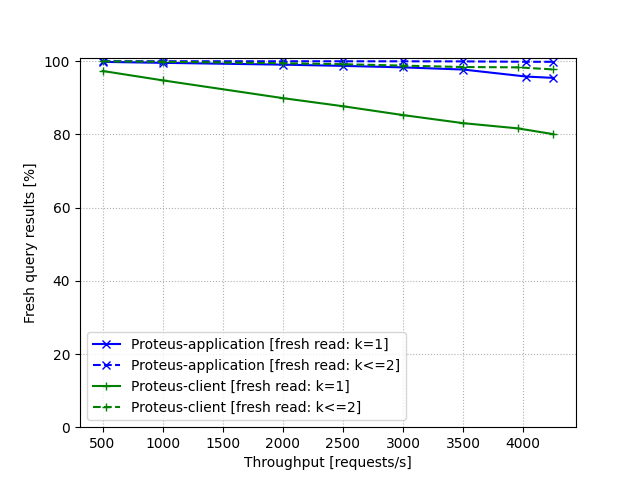
\includegraphics[width=0.7\textwidth]{./figures/evaluation/fresh_reads_throughput.png}
  \caption{Throughput vs percentage of query results and that return a fresh version.
  A returned result is considered fresh if 1) it is the most up-to-date version committed in the database at that time (k=1),
  2) it is amongst the two most up-to-date versions committed in the database at that time (k$\leq$2).}
  \label{fig:fresh_reads_throughput}
\end{figure}

\bigskip
\noindent
Figure~\ref{fig:fresh_reads_throughput} shows the freshness of query results as throughput increases,
measured as the percentage of query results that returned fresh versions.
We define a returned result as a single story with its vote count;
Each front page request returns 25 stories, and each is considered separately.
We consider a scenario in which only the most latest version is considered fresh (k=1),
and one in which the two most recent versions are considered fresh (k$\leq$2).

We observe that:
\begin{itemize}
  \item Proteus-application outperforms Proteus-client, as expected.
  For the k=1 scenario, over 95\% of reads observe the latest versions under the highest load.
  For the k$\leq$2 scenario, freshness remains nearly constant at over 99\%.
  \item Freshness in Proteus-client decreases as throughput increases.
  Proteus-client suffers from up to 80\% stale query results (for k=1), and freshness decreases constantly as load increases.
  However, most stale results observe the second most up-to-date version:
  However, in the k$\leq$2 scenario over 97\% of query results are fresh.
\end{itemize}

These results can be explained using Figure~\ref{fig:fr_latency_throughput}.
In Proteus-client, it takes at lest 45ms for an updated vote count to be reflected in the materialized view,
but a front page request reaches the view with significantly lower delay.
When load is low, this does not lead to stale query results because there are a few vote requests (5\%).
However, as load increases, queries observe increasingly more stale materialized view  entries.

This is not the case for Proteus-application.
There, both types of requests reach the materialized view with similar delay,
and because of the query-heavy nature of the workload,
most queries observe tha latest materialized view entries.

\begin{figure}[H]
\centering
  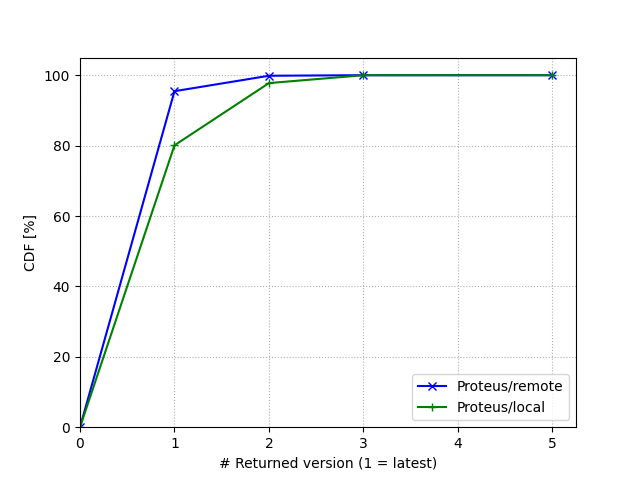
\includegraphics[width=0.7\textwidth]{./figures/evaluation/readV_cdf_throughput.png}
  \caption{CDF of returned version at 4250 requests/s for the Proteus-application and Proteus-client deployments.}
  \label{fig:readV_cdf_throughput}
\end{figure}

Figure~\ref{fig:readV_cdf_throughput} displays a CDF showing how stale a result of a front page request is
(measured in number of versions),
under a load of 4250 requests/second, for the Proteus-application and Proteus-client deployments.
Results show that:
\begin{itemize}
  \item In both deployments, most queries return the latest or second most recent version.
  \item Proteus-application outperforms Proteus-client:
  Under the same conditions, Proteus-application exhibits 4.5\% stale returned results,
  while Proteus-client 20\% (4.4X).
  However, in Proteus-client only 2.2\% of queries results are more stale than the second most recent version.
\end{itemize}

\medskip
\noindent
\textbf{Conclusion.}
Placing the materialized view close to the client, and thus away from the underlying datastore incurs a freshness penalty:
queries return stale results relative to the results that would have been obtained by querying the database.
However, for the workload characteristics in these experiments,
query results rarely more stale than the second most recent version.
Moreover, update latency and versions freshness scale well as the system's load increases.


\subsection{Freshness and round-trip latency}
\label{sec:eval_freshness_rtt}

The experiments in the previous section evaluated the effect of the query processing state placement under a constant
round-trip delay, as the load offered to the system increases.
In this section, we invert these two variables:
we measure freshness under a constant load,
as the (simulated) round-trip time between the application and client site increases,
for the Proteus-client deployment.
The aim of this experiment is to examine the effect of round-trip delay in freshness.

Experiments are performed under a load of 2000 and 4000 requests/second.
We have selected these values based on the results shown in Figure~\ref{fig:fr_latency_throughput}:
Under a load of 2000 requests/second both deployments are able to keep up with the offered load,
while under 4000 requests/second the Proteus-application scheme exhibits increased update latency.

\begin{figure}[H]
\centering
  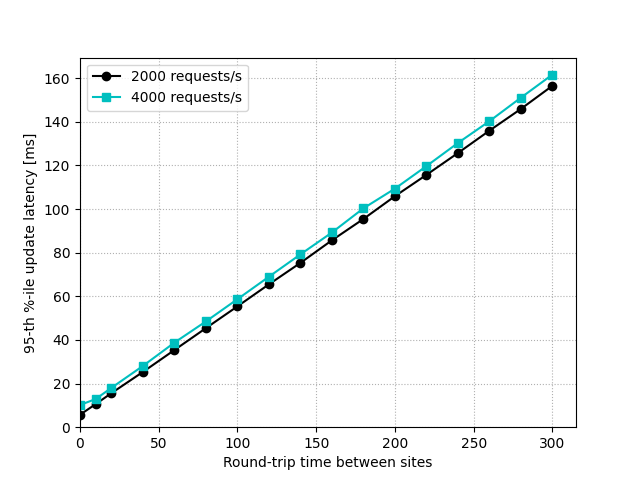
\includegraphics[width=0.7\textwidth]{./figures/evaluation/fr_latency_net_latency.png}
  \caption{Round-trip time between sites vs 95th percentile update latency, for the Proteus-client deployment.}
  \label{fig:fr_latency_net_latency}
\end{figure}

Figure~\ref{fig:fr_latency_net_latency} shows the update latency as the round-trip time between the two sites increases,
under 2000 and 4000 requests/second.
We observe that for both loads, update latency scales linearly with the round-trip time.
Under 2000 requests/second, update latency is at most 5ms above the lower bound set by the one-way network latency
between the two sites, while under 4000 requests/second it is at most 11ms (2.2X).

\begin{figure}[H]
  \begin{subfigure}{0.5\textwidth}
    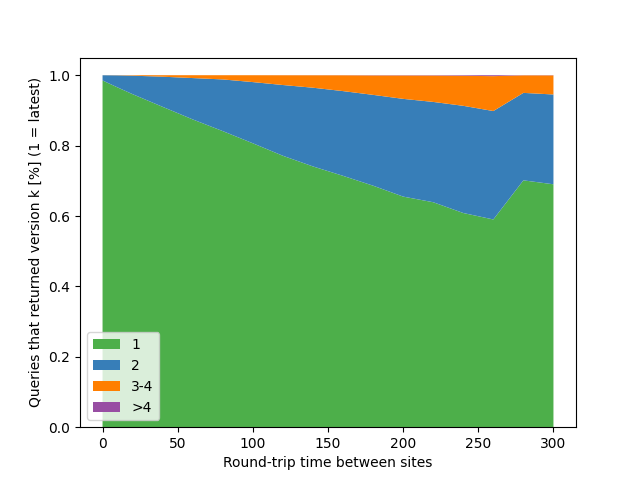
\includegraphics[width=\linewidth]{./figures/evaluation/readV_freshness_netLatency_200.png}
    \caption{2000 requests/second.}
    \label{fig:readV_freshness_netLatency_200}
  \end{subfigure}%
  \hspace*{\fill}
  \begin{subfigure}{0.5\textwidth}
    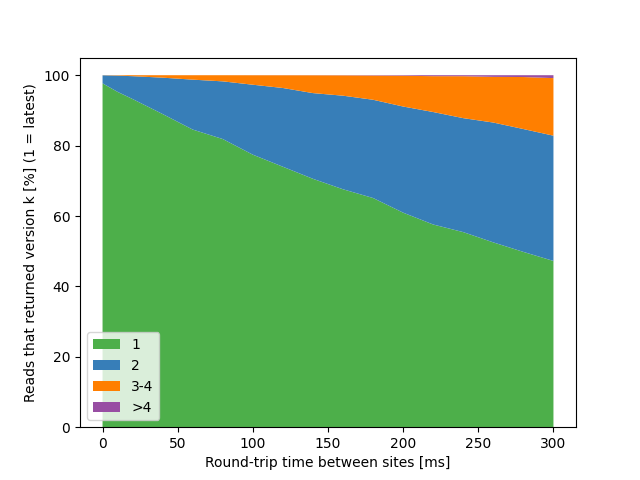
\includegraphics[width=\linewidth]{./figures/evaluation/readV_freshness_netLatency_400.png}
    \caption{4000 requests/second.}
    \label{fig:readV_freshness_netLatency_400}
  \end{subfigure}%
\caption{Round-trip time between sites vs distribution of returned version.}
\label{fig:readV_freshness_netLatency}
\end{figure}

Figures~\ref{fig:readV_freshness_netLatency_200} and~\ref{fig:readV_freshness_netLatency_400}.
We observe that under both loads freshness decreases as round-trip time increases;
Increasing the load of the system increases the gradient of this decrease.
However, in both cases, queries, most of the time, observe at most the forth most recent version:
Only 0.06\% and 0.8\% of query results are more stale than the forth most recent version.

\medskip
\noindent
\textbf{Conclusion.}
Update latency, and the freshness of query results are primarily affected by
by round-trip time between sites,
and to a lesser degree by the system's load.

\section{Data transfer between sites}
\label{sec:eval_data_transfer}
Distributing a query engine across multiple sites entails data transfer between sites.
If the system is deployed on a public cloud platform, this incurs an additional cost,
because data transfer between data centers is part of public clouds' pricing models.
For example, on AWS EC2, data transfer costs \$0.02 per GB \cite{aws:pricing}.

In the scenario used for these experiments, placing the Materialized view QPU at the client site entails that
update records from the Sum to the Materialized view QPU are sent between sites.

To measure the amount of inter-site data transfer,
we have implemented a mechanism for measuring and aggregating the size of outgoing messages at each QPU.
For a 5 minute benchmark, with 4000 requests/second (200 votes/second), 7.7MB of data were transferred between data centers.
This is because only 5\% of requests are votes, and the size of an update record is small (around 90 bytes),
as it only contains the id and vote count of a story.

In contrast, in the same benchmark, 7.5GB of data were sent as query responses.
This is because the size of a query response is around 4MB
(it contains the records of 25 stories), and 95\% of requests are queries.

We conclude that, in this the evaluation scenario, the materialized view can be placed in the client site without incurring
significant data transfer costs.

\section{Conclusion}
\todo{evaluation conclusion}
% \section{Navigating the design space of geo-distributed query}
% (Note: The title might be a bit too fancy. To re-think.)

% Question to answer:
% Can the QPU approach be used to adjust to navigate the design space
% geo-distributed query, making different trade-offs depending on the requirements
% and characteristics of specific applications.

% Hypothesis to validate:
% For a given pair of workload type (eg. query-heavy) and requirement (expressed
% as performance/efficiency metric) there is a query engine configuration that
% ''optimizes'' the given metric.

% (Idea on how to visualize this: 2D matrix ''workloads - metrics'':
% for each cell, find which configuration is best for this workload and metric.

% High-level plan:
% \begin{itemize}
%   \item Run a set of different workloads, measuring different metrics (query
%   performance, freshness, cost)
%   \item Repeat this for a set of query system configurations.
%   \item Examine for each worload-metric pair, how changing the query engine
%   configuration affects the target metric.
% \end{itemize}

% \section{Application benchmark}
% (Note: I ran out of inspiration for titles)

% Question to answer:
% What performance gains can the QPU approach deliver to an application, and how
% it Proteus compare against state-of-the-art systems?

% Hypotheses to validate
% \begin{itemize}
%   \item 1. The QPU approach (Proteus) can provide the performance comparable to
%   that of state-of-the-art systems when used with a similar configuration.
%   \item 2. The QPU approach (Proteus) can improve the application's performance
%   (or improve freshness or cut cost) by enabling query engine designs (placement
%   schemes, ...) not possible with current query systems.
% \end{itemize}

% (This is currently being designed and implemented.)